\documentclass[a4paper, two column]{article}

\usepackage[utf8]{inputenc}
\usepackage{multicol}
\usepackage{amsmath}
\usepackage{amsfonts}
\usepackage{tikz}
\usepackage{graphicx}
\usepackage{mdframed}
\usepackage{color}
\usepackage{listing}
\usepackage{wrapfig}
\usepackage[parfill]{parskip}
\usepackage{subcaption}
\usepackage{hyperref}
\usepackage[font={small}]{caption}
\usepackage{marvosym}
\usepackage[margin=0.7in]{geometry}
\usepackage{tablefootnote}
\usepackage{abstract}
\usepackage{enumerate}
    \makeatletter
    \let\@fnsymbol\@arabic
    \makeatother
\begin{document}
\twocolumn[{
\centering
{\LARGE \textbf{GPU-accelerated facet-based convolutional gridding}}\\
{\large \textbf{The problem of non-coplanar widefield imaging in radio astronomy}}\\
Benjamin Hugo\thanks{bennahugo@aol.com}\\
Supervised by: James Gain\thanks{jgain@cs.uct.ac.za} and Oleg Smirnov\thanks{osmirnov@gmail.com}\\[0.5cm]
}]
\saythanks
\section{Introduction}
\subsection{Problem Context}
Modern radio astronomy observes electromagnetic emissions from black bodies and magnetic processes with wavelengths typically around one million times longer than that of visible light, and is subsequently 
able to observe phenonma that is invisible at the wavelengths of visible light. Since its birth in the early 20th century, research has been largely driven towards building telescopes with higher resolving capability. 
In modern radio astronomy this is achieved through aperture synthesis. In essence this process combines the resolving capacity of smaller apertures to provide an equivalent
resolving capability to that of a single very large aperture. This is achieved by taking short time averages between the outputs from pairs of antennae, through a process known 
as signal correlation \cite{christiansenradiotelescopes,taylor1999synthesis}. 

Each antennae pair in such an array samples the sky in the Fourier domain, and an image of the sky can be obtained through Fourier inversion of all these ``visibility'' samples. See figure~\ref{FIG_APERTURE_SYNTH}. One technique commonly employed is that of convolutional gridding and 
Fast Fourier Transforms. This approach approximates an area on the celestrial sphere by a tangent plane and is typically about two orders of magnitude faster than computing each image pixel directly \cite[Lecture 7]{taylor1999synthesis}, especially when 
considering large visibility datasets. As telescope arrays grow larger, the size of these datasets grow quadratically with the number of elements of the array. Coupled with the problems of telescope calibration and image deconvolution, which may take several cycles of 
convolutional gridding and degridding, accelerating the imaging process is of vital importance in large arrays such as LOFAR and the Square Kilometer Array.

\begin{figure}[h]
 \begin{mdframed}
 \centering
 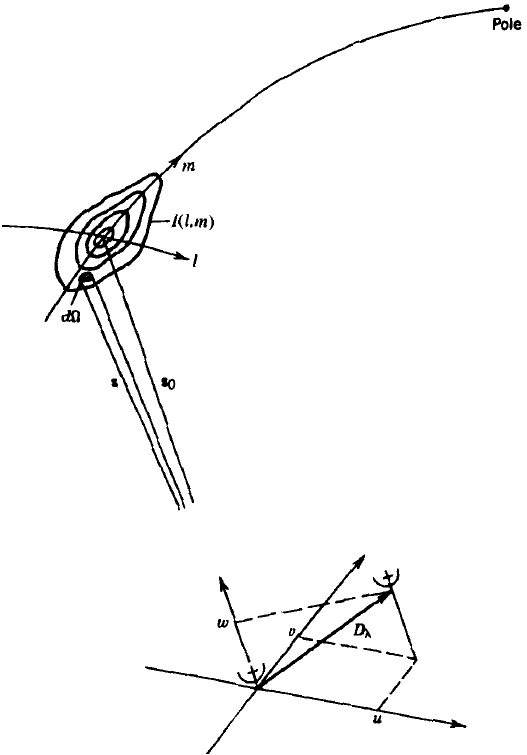
\includegraphics[width=0.8\textwidth]{lmn_uvw.png}
 \caption[The relation between image space and visibilities]{The relation between the measured sampled visibility function (u,v,w space) and the projected source on the unit ``celestial'' sphere (l,m,n space). Image taken from Synthesis Imaging II \cite{taylor1999synthesis}.}
  \label{FIG_APERTURE_SYNTH}
 \end{mdframed}
\end{figure}

Both convolutional gridding and its inverse, convolutional degridding, can be parallelized and is suitable for processing on massively multicore architectures such as General Purpose GPUs. Although convolutional gridding 
has been implemented on GPUs in past research (for example \cite{romein2012efficient}), the grid sizes required by the Square Kilometer Array cannot easily be fitted in the onboard memory of current GPU accelerators. This problem can be mittigated by facet-based
imaging, where each image is split into multiple smaller facets, and computed independently of eachother. 

This image-based faceting approach is described by Cornwell and Perley \cite{cornwell1992radio} and involves dividing the celestial sphere into small approximating planes (in other words the sphere is approximated by a polyhedron). 
As normal convolutional gridding is only useful to approximate small areas on the sphere, the use of facets, w-projection \cite{cornwell2005w} or snapshots (a series of short-time observations) is 
necessary to facilitate imaging wide fields of view. This is especially true at low frequencies, like those observed by LOFAR. 

The associated problem of imaging using non-coplanar baselines significantly worsens the distortions (see figure~\ref{FIG_3D_DISTORTIONS}) caused by gridding large fields of view. In non-east-west two-dimensional arrays the 
Earth's rotation slowly rotates the vector direction between two telescopes (a ``baseline'') through multiple heights. Although corrective W-projection can be integrated into convolutional gridding, and is known to be significantly faster than facet-based approaches, faceting has lower memory requirements 
than computing the entire image in a single step. Faceting is therefore a more feasible approach for large arrays such as the Square Kilometer Array. The additional computational demands of faceting can be significantly reduced if the celestial sphere is only sparsely imaged. In this situation the majority
of the facets are concentrated around sources, while the rest of the image is not computed. This is known as ``targetted'' faceting.

\begin{figure}[h]
 \begin{mdframed}
 \centering
 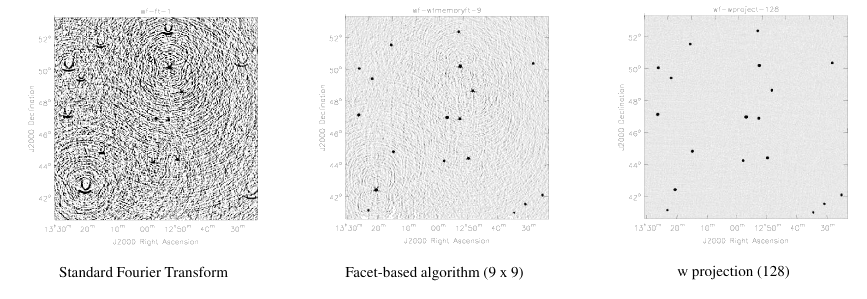
\includegraphics[width=0.5\textwidth]{3d_correction.png}
 \caption{The distortions caused by widefield imaging without corrections (standard Fourier transform) and with 3D corrections (faceting and w-projection). Image by Cornwell et al. \cite{1416440}}
  \label{FIG_3D_DISTORTIONS}
 \end{mdframed}
\end{figure}

A third benefit to faceting is the removal of time-invariant (or slowly variant) directionally dependent effects \cite{2011A&A...527A.107S}. The slow-varying directional dependent effects, such as those introduced by the 
ionosphere and antenna beam patterns can be approximated over small facets and subsequently removed. The effects are modeled as a set of Jones matricies \cite{2011A&A...527A.106S}, whose inverses are applied to the output of each antenna. Because these terms are locally invarent over small 
facets, they can be corrected for before convolutional gridding. The general relation between the image space and the sampled coherence function is given by the measurement equation (equation~\ref{eqn_RIME}). In a facet-based approach
the directionally dependant effects is moved out of the integral, provided the facets are small enough.

\begin{figure*}
\begin{mdframed}
\begin{equation}
\label{eqn_RIME}
\begin{split}
    V_{pq}(u,v,w) &= G_p(t,\upsilon)\left(\int_{-\infty}^{\infty}\int_{-\infty}^{\infty}D_p(l,m,t,\upsilon)BK_{pq}D_q(l,m,t,\upsilon)^H\frac{dldm}{\sqrt{1-l^2-m^2}}\right)G_q(t,\upsilon)\\
	  &\text{where }K = e^{-2\pi i(u_{pq}l+v_{pq}m+w_{pq}(n-1))}
    \left[\begin{array}{c c}
     1 & 0 \\
     0 & 1 \\
    \end{array}\right]\\
	 &\text{and the G terms are the direction-independent effects,}\\
	 &\text{while the E terms are dependent on the direction of the source in l,m space}\\
 	 &J^H:=\bar J^T \text{ indicates the Hermitian transpose (the transpose of a complex conjugate matrix)}\\ 
 	 &\text{if }w(n-1)\approx 0\text{ the relation is an ordanary 2D Fourier transformation}
\end{split}
\end{equation}
\end{mdframed}
\end{figure*}

Faceting has been the defacto standard in the Astronomical Image Processing System (AIPS) task ``IMAGR'' \cite{AIPS113} when it comes to imaging fields of view, and is still 
widely used in newer toolkits such as the Common Astronomy Software Applications (CASA) \footnote{Freely available from \url{casa.nrao.edu}}. 

\subsection{Research objectives}
Our research aims to achieve the following key objectives:
\begin{enumerate}[i)]
 \item \textbf{Implement an optimized CPU-based faceted convolutional gridder in C++}\\
  This will be achieved using OpenMP and AVX vector intrinsics where applicable. It will serve as a reasonable baseline for performance comparisons of a GPU-based version and previous research.
 \item \textbf{Implement a GPU-based faceted convolutional grider in CUDA}\\
  The GPU version will be based on the most work-efficient GPU gridding algorithm in the literature, but will modified to include faceting instead of w-projection.
 \item \textbf{Create a distributed solution using the Message Passing Interface}\\
  The sheer scales of these tasks ensures that both a purely parallel CPU version and a GPU version of the faceted gridder can benefit from additional computing power offered by even that of a small cluster.
\end{enumerate}

The chapter on methodology deals with validation and performance metrics. We will consider the project successful if the distributed GPU imager is substantially faster (40-50x) compared to (optimized) CPU-based 
faceted imaging.
\section{Literature review}
 Both convolutional gridding and faceting are well-understood problems. Convolutional gridding (throughly detailed in Synthesis Imaging II \cite{taylor1999synthesis}) is not only used in radio astronomy, but in other fields such as 
 medical imaging as well (see for example Jackson et al. \cite{jackson1991selection}). Although it is possible to do faceting on both separate image-space planes \cite{cornwell1992radio} or a single plane as with so-called ``uv-facets'' \cite{AIPS113}, we opted to support targeted 
 faceting by faceting in the image space. If the entire image is faceted in a full-image faceting mode of operation, the facets have to be joined into a final image, once they have been deconvolved, degridded, corrected for amplitude and phase error and regridded over several iterations. 
 This operation is well-understood and is implemented in the FLATN task in classical AIPS. The image space transformation is discussed by Sault et al. \cite{sault1996approach}.
 
 In order to use an Inverse Fast Fourier Transform between the sampled ``visibilities'' and the image, one first has to sample the visibilities onto a regular grid. Convolutional gridding takes each visibility (per frequency channel, time step and baseline) 
 and interpolates it onto a grid. The interpolation is achieved by multiplication with a convolution function. When antenna polarization is taken into account there can be up to 4 separate grids onto which these visibilities are sampled. In this research we will
 use the optimal gridding convolution function approximation of Sze Tan \cite{tan1986aperture}. Here ``optimal'' is defined in terms of minimizing aliasing energy outside the gridded area and minimizing the interpolation error between gridding and the brute force per-pixel
 imaging (also known as the ``Direct'' Fourier Transform).
 
 The co-planar convolutional gridding algorithm and Fast Fourier Transform has a combined complexity of $O(MC^2) + O(N^2\log_2{N})$, where M is the number of observed visibilities, N is the size of one of the grid dimensions and C is the size of one of the convolution kernel 
 dimensions. For long observations $M\approx N^2$. This is still much faster than the direct approach which has a complexity of $O(N^4)$. When faceting is added to the gridding algorithm it can fast become computationally prohibative to do a completely faceted image. In both directions 
 the number of facets required is approximately $N_{poly}=2B_{max}\lambda/fD^2$, where $B_{max}$ is the length of the longest baseline, $D$ is the the diameter of the antennae reflectors and $f << 1$ \cite{taylor1999synthesis}. It should be said that this approach is typically
 still less memory intensive than gridding several height planes and taking a three-dimensional Fast Fourier Transform. It is also less memory intensive and faster than directly computing each voxel \cite{yashar2009tdp}. Cornwell et al. \cite{1416440} points out that for low-frequency observations (74 MHz) 
 faceting is typically around an order of magnitude slower (seconds) than w-projection.  See figure~\ref{IMG_PERFORMANCE_COMPARISON} for a comparitive plot.
 \begin{figure}
 \begin{mdframed}
  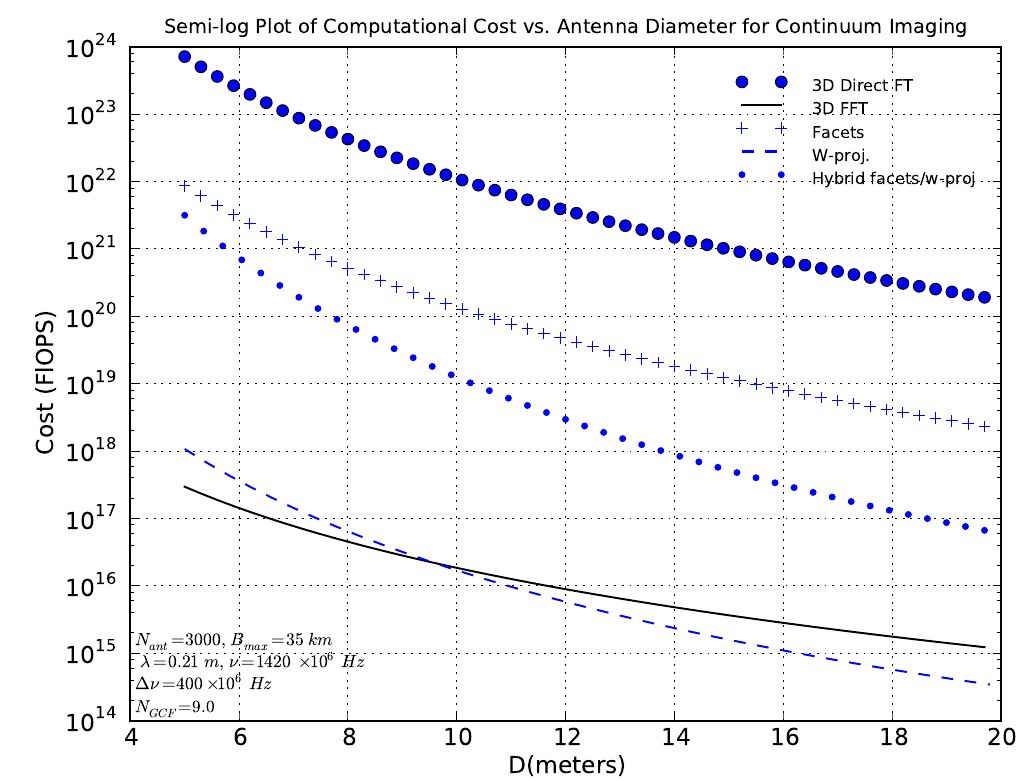
\includegraphics[width=1.0\textwidth]{performance_faceting.png}
  \caption{Plots of computational cost (floating point operations per second vs. antenna diameter D) of several schemes including w-projection and hybrid faceting and w-projection. Image taken from an analysis by Yashar and Kemball \cite{yashar2009tdp}.}
  \label{IMG_PERFORMANCE_COMPARISON}
 \end{mdframed}
 \end{figure}

 As one may expect, this convolutional gridding requires atomic operations when parallelized. Romein \cite{romein2012efficient} suggests a novel approach which limits the number of atomic operations required by a GPU gridding process, by accumulating
 the contribution to each grid cell in registers. This approach outperforms all other parallel gridding approaches, including presorting, but suffers from convolution function weight lookups and GPU memory size for large images \cite{muscat2014high}.
 A faceting (or at minimum, a hybrid faceting and w-projection) approach is currently necessary to mitigate the latter. It is estimated that the images produced from observations on the SKA may contain up to $10^{10}$ pixels \cite{cornwell2012wide}. 
 If each grid is to be computed using single precision floating point aritmetic this will amount to 37.25 GiB of GPU memory on storing the grid for a single polarization average. Storing the visiblity data, Fast Fourier Transformation and the possible 
 storage of convolution kernels will require additional memory. 
 
 According to Cornwell and Perley \cite{cornwell1992radio} image-space faceting requires phase shifting (multiplying with a complex exponential) each visibility to the facet center and rotating each facet in order to 
 be tangential to the sphere at the facet center. This transformation is achieved by a simple 3x3 rotation matrix, as is done in IMAGR \cite{AIPS113} and is necessary to avoid additional distortions in the field of view \cite[pg. 395]{taylor1999synthesis}. To the best of our knowledge 
 a faceted convolutional gridder has not yet been implemented on GPUs, although Golap et al. \cite{golap2001parallelization} has made some effort in parallelizing facet imaging, facet deconvolution and re-projection onto a common tangent plane.
 
 Any parallel work-distribution strategy that involves faceting will not be as simple as convolving visibilities onto a set of grids. Because these grids are typically comparitively small, the majority of the uv-coverage will fall outside the grid being processed. This will cause 
 excessive branch divergence and will subsequently be very slow. We propose that the visibilities be ``binned'' according to the facets that they contribute to. This will ensure that both global memory accesses and branch divergence is kept to a minimum. Each group of threads will
 work on a particular grid, where each thread monitors strided grid locations, but maintains coalesced memory access patterns. This is in accordance to the access pattern put forward by Romein \cite{romein2012efficient} and minimizes atomic accesses by making use of the plentiful fast 
 register memory on current GPUs. The facets and associated visibility information can then be distributed accross multiple GPUs, ensuring course-grained parallelization.
\section{Methodology}
\subsection{Research design}
The focus of this research is not on generating new methods of imaging, but merely accelerating the widely known and used method of facet-based synthesis imaging. The novelty of the research undertaken lies in solely in the acceleration
of a previous algorithm. To the best of our understanding the problem is suitable for GPU acceleration, and our research simply aims to explore this approach to imaging as a viable solution to the memory requirement constraints of current techniques.

The research process will be split up into 3 distinct phases:
\begin{enumerate}
 \item Phase 1 deals with algorithm development, and is done in Python. The full faceting, gridding and FFT processs is implemented to ensure that the validity of the approach (discussed shortly). This phase is already underway at the time of
       submitting this proposal.
 \item Phase 2 will focus on developing an optimised and distributed CPU version.
 \item Phase 3 will consist of the development of an distributed optimized GPU version in Nvidia CUDA.
\end{enumerate}

\subsection{Performance metrics}
Previous gridding litterature \cite{muscat2014high,romein2012efficient} has made comparisons in terms of ``Gigagridpoint additions per second'' and we will measure the same performance metric in order to judge whether the gridder is on par with those described 
in the litterature. The measure of throughput (size of input visibilities / total seconds to grid facets) can be used to judge how well the implementation is using available GPU memory bandwidth (which is typically more than an order of magnitude slower than the 
floating point processing capability of modern GPUs). This assumes the processing time computing each facet significantly outweighs the cost of transferring memory to and from the GPU.

Throughput will likely be one of the most important performance metrics. This metric may be more substantial for measuring gridding performance on GPUs compared to measuring performance 
as floating point operations per second. The reason is that the the performance of convolutional gridding can be considered to be a memory bound problem. Typically each global memory access may take hundreds of clock cycles, compared to only a few clock 
cycles per arithmetic operation. Arithmetic intensity (number of operations performed per byte accessed in memory \cite{sclocco2014auto}) gives a good estimation whether the algorithm will be compute or memory bound. To obtain good GPU performance 
the arithmetic intensity has to be high. Convolutional gridding does not involve a significant amount of arithmetic per global memory access, and can therefore not exploit the peak computational capability of a GPU. Although faceting adds additional complex 
exponentiations and coordinate transformations to each visibility, it also adds additional memory accesses. We believe that faceting will not substantially alter the arithmetic intensity and 
the problem will remain memory bound.

Substantial parallelization may translate to speedups which can mean the difference between hours and possibly minutes of computation for a single image. Targetted faceting over sparse images (described in the litterature review) will
be the optimal situation for using an acceleratated faceting approach, since this will significantly reduce the amount of computation time involved with creating an image. 
\subsection{Data sources}
Obtaining real observation data and reading these datasets for performance benchmarking will not be a problem. We have access to vast amounts of data, as well as well-tested and documented third party libraries which can read and convert between
popular formats.
\subsection{Validity}
 To ensure that the images produced by our gridder are correct they will be compared to the dirty images produced by well-known radio imaging toolsets which supports three-dimensional correcting techniques (ie. w-projection or faceting). CASA satisfy these requirements and is easy to use. In order 
 to perform this validation this it is possible to generate a large synthetic dataset with several point sources in order to test the output of the faceted gridder.
\subsection{Resources required} 
 This project will not require substantial resources beyond the use of the UCT High Performance HEX cluster (or possibly the cluster at the Center for High Performance Computing). It may be possible to also benchmark the algorithm performance
 on newer hardware such as the Tesla K10 on the Amazon EC cloud for a small hourly fee (\$0.650 USD \footnote{Available from \url{http://aws.amazon.com/ec2/pricing/}. This is the quoted price at the time of writing (9 May 2014 9:33 am).}). For development purposes we have access to a Nvidia GeForce 
 GTX 770 and a 4th generation Intel i7 CPU with support for the AVX 2.0 instruction set. This research will not require any ethical clearence and poses no substantial risk.
\section{Work plan}
A brief schedule is given below:\\
\begin{tabular}{|p{2.5cm}|p{5cm}|}
 \hline
 \textbf{Due} & \textbf{Task} \\
 \hline
 30 June 2014 & Prototype of Faceted Gridder and Background chapter\\
 \hline
 31 August 2014 & C++ Implementation\\
 \hline
 31 October 2014 & GPU Implementation\\
 \hline
 7 January 2015 & Optimized GPU Implementation\\
 \hline
 30 March 2015 & MPI implementations and Design Chapter\\
 \hline
 31 July 2015 & Possible experimentation with hybrid faceted w-projection\\
 \hline
 31 August 2015 & Results \\
 \hline
 31 October 2015 & Corrections \\
 \hline
\end{tabular}
{
\bibliography{proposal}
\bibliographystyle{plain}
}
\end{document}
